\hsection{Object Equality and Identity}%
\label{sec:equalityAndIdentity}%
%
\begin{figure}%
\centering%
\begin{tabular}{r@{:~}lr@{:~}lr@{:~}l}%
\multicolumn{2}{c}{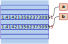
\includegraphics[width=0.275\linewidth]{\currentDir/different}}&%
\multicolumn{2}{c}{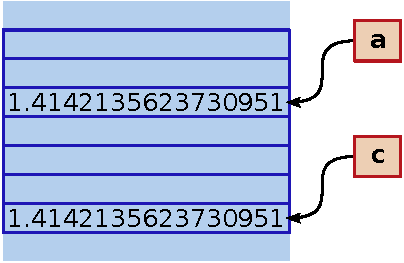
\includegraphics[width=0.275\linewidth]{\currentDir/equal}}&%
\multicolumn{2}{c}{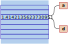
\includegraphics[width=0.275\linewidth]{\currentDir/same}}\\%
%
\pythonil{a == b}&\pythonil{False}&%
\pythonil{a == c}&\pythonil{True}&%
\pythonil{a == d}&\pythonil{True}\\%
%
\pythonil{a is b}&\pythonil{False}&%
\pythonil{a is c}&\pythonil{False}&%
\pythonil{a is d}&\pythonil{True}\\%
\end{tabular}%
%
\caption{A illustration of the concepts of equality (\pythonilIdx{==}) and identity (\pythonilIdx{is}) from the perspective of variables.}%
\label{fig:variables:equalityAndIdentity}%
\end{figure}%
%
\gitPythonAndOutput{\programmingWithPythonCodeRepo}{variables}{identity_1.py}{--args format}{variables:identity_1}{%
An example of the difference between equality and identity\pythonIdx{sqrt}.}%
%
\gitPythonAndOutput{\programmingWithPythonCodeRepo}{variables}{identity_2.py}{--args format}{variables:identity_2}{%
An second example of the difference between equality and identity.}%
%
We use variables to references objects in memory.
When we compare two variables, we actually compare the objects they reference.
It is clear that two variables can reference objects that are either equal or not equal.
They can also reference the same object.
These two concepts -- equality and identity -- must be distinguished.

And this can be done rather easily.
Imagine that you buy a green jacket, let's call it~$A$.
Then you buy the exactly same jacket again, for a second time, and call the second jacket~$B$.
Now~$A$ and~$B$ are equal, but they are still two different objects.%
%
\begin{sloppypar}%
\Cref{fig:variables:equalityAndIdentity} illlustrates this issue.
If we have two variables \pythonil{a=1.4142135623730951} and \pythonil{b=1.4142135623730953}, then they have different values and reference different objects (namely, the two different memory cells holding the two different \pythonil{float} values).
In this case, \pythonil{a == b}\pythonIdx{==} and \pythonil{a is b}\pythonIdx{is} will both return \pythonil{False}.%
\end{sloppypar}%
%
Now we can also have another variable \pythonil{c}, which may reference a \pythonil{float} object that holds the same value as the one referenced by~\pythonil{a}.
This value would be stored somewhere else in memory.
Then, \pythonil{a == b} is \pythonil{True}, because the variables have equal values.
However, \pythonil{a is b} would be \pythonil{False}, because they still reference different objects.

If I would declare a variable \pythonil{d = a}, then \pythonil{d} would point to exactly the same \pythonil{float} object as~\pythonil{a}.
Now, both \pythonil{a == b} and \pythonil{a is b} are \pythonil{True}.

A simple example of the difference between equality and identity is given in \cref{lst:variables:identity_1}.
Here, we declare a \pythonil{float} variable and store in it the value of~$\sqrt{2}$ (as exactly as it can be represented by a \python\ \pythonil{float}, that is), which just so happens to be \pythonil{1.4142135623730951}.
We then import the function \pythonilIdx{sqrt} from the \pythonilIdx{math} module and compute~\pythonil{sqrt(2.0)}.
We store the result of this in a second variable, namely \pythonil{sqrt_2_computed}.
We find that \pythonil{sqrt_2 == sqrt_2_computed} is \pythonil{True}, whereas \pythonil{sqrt_2 is sqrt_2_computed} is \pythonil{False}.
The two values are clearly the same, however, they are stored at two different memory locations.
The interpreter did not know that the same value as the result of \pythonil{sqrt(2.0)} was already stored somewhere in memory.
Therefore, it allocated the necessary memory for the result of the \pythonilIdx{sqrt} operation and stored it there.
We now have two variables that reference two objects which both hold the same value.%
%
\noviceHint{%
In the rest of this subsection, we discuss (albeit superficially) how objects are cached and reused. %
First-time readers are welcome to skip over the rest of this subsection.%
}%
%
A slightly more involved example of the issue of object equality and identity is given in \cref{lst:variables:identity_2}.
You see, when the \python\ interpreter parses the program code file, it will allocate the memory and store the values of constants and literals.
\cref{lst:variables:identity_2}, we declare \pythonil{a = "Hello World!"} and then \pythonil{b = "Hello World!"}.
In other words, \pythonil{a} and \pythonil{b} will receive the same value.
As the output in \cref{exec:variables:identity_2} shows, the \python\ interpreter is clever enough not to store this value twice in memory.
Instead, \pythonil{a} and \pythonil{b} will point to the same object, i.e., \pythonil{a is b} holds.
Interestingly, even if we subsequently do \pythonil{c = "Hello " + "World!"}, the interpreter is still clever enough to recognize that this constant expression yields the same result already stored in~\pythonil{a}.
It basically computes the result of the concatenation of the two constant strings and discovers this identity.
Therefore, \pythonil{a is c} will also be \pythonil{True}.

If we use a variable in such an expression, it does no longer work, though:
First setting \pythonil{d = "Hello"} and then setting \pythonil{d = d + " World!"} will yield an equal result~(\pythonil{a == d} is \pythonil{True}), but it will be stored somewhere else in memory~(\pythonil{a is d} is \pythonil{False}).
The interpreter, at least in its current version, cannot infer value identities of results of computations that involve values that are not constants.

Well, sometimes it can.
It seems that \python, like \pgls{Java}, caches a set of small integers.\footnote{%
Some sources say that all integers between \pythonil{-5} and \pythonil{256} are cached. %
However, this is highly implementation and configuration specific and may be entirely different on your machine.%
}
It is obvious that we need small integer numbers again and again and again in our programs.
Allocating a new objects whenever we use the values \pythonil{1} or \pythonil{0} would be wasteful.
In \cref{lst:variables:identity_2}, we calculate the result of the computation \pythonil{f = (e * mul) // mul}, where \pythonil{e} is a variable with value~\pythonil{10} and \pythonil{mul} is a variable with value~\pythonil{5}.
The result is obviously \pythonil{10} as well, i.e., a small integer.
And it is identical to~\pythonil{e}, i.e., \pythonil{e is f} is \pythonil{True} -- despite begin the result of a computation including only variables.

We now replace \pythonil{10} with a large value, say we set~\pythonil{g = 1_000_000_000_000_000_000}.
We compute \pythonil{h = (g * mul) // mul}.
Of course, \pythonil{g == h} is \pythonil{True}.
However, \pythonil{g is h} is \pythonil{False}.
Because this integer value is too large to be cached and a new object is generated.%
%
\FloatBarrier%
\endhsection%
%
